\chapter{Analysis}
\label{chapter:analysis}

In \autoref{cha:prior-work}, we discussed how the project started as a decentralized
storage system with verification and then evolved into integrating PoR into the verification,
as soon as limitations of the decentralized verification mechanism were discovered.
In this chapter we will discuss how we are solving the problem of storage attacks
and how PoR integrates into the reputation system.
It is worth noting that apart from malicious peers, it is also possible for well-behaved peers to
lose data due to hardware failures and bit rot.
We will not cover this case as a special case, because it is a light version of what malicious
peers are capable of doing.

\section{Malicious peers}

There could be many types of malicious peers in a decentralized network,
but we will cover only the relevant ones for the scope of the project.
The Related Work \autoref{chapter:related-work} covers other systems and
how they handle the other types of attacks, not covered here.

There are two types of scenarios that can affect the integrity of the data in the network:
\begin{enumerate}
    \item \textbf{Data availability degradation} --- an attacker claims to store data, but does not.
    \item \textbf{Data integrity degradation} --- an attacker claims to store data, but stores different data, or
        data that has become corrupted without the peer being necessarily malicious.
\end{enumerate}

While the two seem similar, we will cover them separately, because they are performed by different types of attackers
and the detection mechanisms are different.
We would like to investigate the different behaviors of peers and how to deal with them.
How severe should the punishment for each type of attack be?

\textbf{Data availability degradation} could be caused by the following peer behaviors:
\begin{enumerate}
    \item \textbf{Not storing the data} --- the peer does not store the data at all.
    \item \textbf{Peer goes offline permanently} --- the peer goes offline at some point in the future after accepting to store the data.
    \item \textbf{Peer goes offline temporarily} --- the peer goes offline for a short period of time.
        This could be a peer that is restarting or lost connection to the network.
        This is not necessarily a malicious peer, but it should be accounted for,
        because malicious peers could be performing an eclipse attack.
    \item \textbf{The peer is slow to respond} --- the peer is slow to respond to requests.
        This could happen when a peer is overloaded or has a slow connection.
        It could also be a malicious peer that is not storing the data and tries to request it
        from another peer in the network, before answering the request.
\end{enumerate}

\textbf{Data integrity degradation} could be caused by the following peer behaviors:
\begin{enumerate}
    \item \textbf{Storing corrupted data} --- the peer stores corrupted data.
        It could be that the peer is trying to save space by storing partial data
        or is trying to disrupt the network.
        Or perhaps the data has become corrupt over time without the peer being malicious.
    \item \textbf{Storing corrupted metadata} --- the peer stores the correct data, but the metadata is corrupted.
        This could mean storing the wrong expiry date or the wrong key.
        This kind of behavior either wouldn't affect the operation of the network or it would fall
        under the other types of behaviors.
        For example, if the peer is storing the wrong key, it would be the same as not storing the data,
        as querying for the original key would result in no response.
\end{enumerate}

The impact of all of these behaviors on the network is always dependent on the time it takes to detect them.
If the time to verify a piece of data is too long, a malicious peer could delete it and then
request it from another peer in the network just before the audit.
Thereby passing the audit, but not contributing to the network.
While this is a possible attack, it is an expensive one to execute,
because the attacker needs to perform a lot of work to pass the audit.
The attacker also needs to contribute considerable amount of their bandwidth to execute such an attack.
This is precisely the reason why we want lightweight audits for the auditor and heavier audits for the auditee.
For the above reasons, we will not consider this attack in our analysis.

\section{Using Proof of Retrievability (PoR) to prevent attacks}

Preventing a Data availability attack can be done by querying the peer whether it has the data.
In this case we assume that the peer is honest and will return a simple answer whether it has the data or not.
The assumption that a peer will be honest is naive, but allows us to easily check if the peer is responsive.
One of the reasons we want to separate this attack is, so we can analyze peers going offline separately.
We will discuss how to handle temporary and permanent offline peers in the evaluation section.

Preventing a Data integrity attack can be done by requesting the peer to return the data and checking if
the data is correct.
This is a costly operation, because the data could be large, and the network could be slow.
This is a stronger requirement for the network, because peers performing this attack are a superset
of the peers performing the data availability attack.

In order to address data integrity attacks, we make use of Proof of Retrievability (PoR).
PoR is a cryptographic protocol that allows a peer to prove to a verifier that it is storing a file.
The verifier does not need to know the file, but only a small secret that is generated from the file.
The verifier can then challenge the peer to prove that it is storing the file by sending a challenge and
comparing the response to an expected response.
Both the challenge and the response are small.
The exact size depends on the PoR protocol used, and in our case is $O(\sqrt{N})$ \cite{poralgebra} for
both the challenge and the response, where $N$ is the size of the file in bytes.

Since the PoR protocol is cheap to execute both on the network and on the computation side of the verifier,
it can be used to address both types of attacks.

\section{Reputation system}

To keep track of the behavior of the peers in the network, we will use a reputation system.
In short, we want well-behaved peers to have a high reputation and malicious peers to have a low reputation.
Also, well performing peers should have a higher reputation than poorly performing peers.
e.g., a peer that responds slowly or fails audits because their hard drive malfunctioned should
have a lower reputation than a peer that is always online and responds quickly to requests.
While this might seem punishing to the peer that has a malfunctioning hard drive,
it is important to keep the network healthy and to prevent the peer from causing more damage to the network.
Peers with higher reputation will be prioritized by the network, while peers with lower reputation will be
avoided and potentially removed from the network.
A key part of designing the reputation system is defining how much reputation is adjusted in each case.
First, we will look into what situations lead to reputation adjustment, and then we will
analyze how much reputation should be adjusted in each case.

Reputation will be increased when a peer is behaving as expected,
i.e., storing data and providing data, as well as performing audits will lead to an increase in reputation.

Reputation should be decreased in the case of failure to comply with the network rules.
A peer that is not storing data should have their reputation reduced on each audit,
until their reputation is so low that they are not trusted anymore and are removed from the network.
A peer that goes offline permanently would fall under the same category, as it would fail all its audits.
A peer that goes offline temporarily should be punished for the failed audits,
but the punishment should be such that for a short period of being offline the peer should not use 
too much of its reputation.
When a peer is slow to respond to requests, the audit will be considered failed and the peer will have
its reputation reduced as if it was not storing the data.

For the data integrity attacks, and in particular for storing corrupted data,
the punishment should be the same as for the data availability attacks.

The questions we need to answer are:
\begin{enumerate}
    \item How many audits can we perform in parallel?
    \item What is the performance impact of the audits on the network?
    \item How do we balance the punishment so that a peer that has been offline for a short period of time
        is not punished too much?
    \item What is a short period of time to be offline?
    \item Can we make the punishment scale with time? The longer the peer is offline, the more severe the punishment.
    \item What does it mean for a peer to be slow to respond?
\end{enumerate}

We have mostly answered the last question in our previous work, where we have evaluated the performance of
the PoR scheme we have implemented.
For small enough files, we cannot guarantee that the peer is storing the data
and not just fetching it from another peer in the network.
But to answer the question fully, we also need to account for the network latency.
If we look at the ping times between London, UK and Christchurch, New Zealand,
we can see that the average ping time is around 275ms \cite{pingtimes}.
These two cities give us a rough estimate of the maximum distance between two peers in the network,
as they are on the opposite sides of the globe.
These results are achieved under ideal conditions, and the actual ping time could be much higher.
We propose 500ms as the maximum time a peer can take to respond to a request.
This is almost 2 times the average ping between two very distant cities, so it should cover all cases.

This time is not accounting for the time it takes to process the request, but only the time it takes for the
request to reach the peer.
The time to process the request is the sum for reading the file from disk and executing the PoR protocol.
The time to execute the PoR protocol is around 40ms for a 100 MB file as our benchmarks show in \autoref{fig:por-keeper}.
The time to read a 100 MB file from disk is around 14ms on an SSD and 200ms on an HDD, if we
use the average read speed of 7000 MB/s for an SSD and 500 MB/s for an HDD.
Assuming that most peers use HDD for cheap storage, we will use the 200ms time to read a 100MB file from disk.
Adding these up, we should expect a Keeper's response to take 500ms + 250ms for each 100 MB of data.

\begin{figure}
  \myfloatalign
  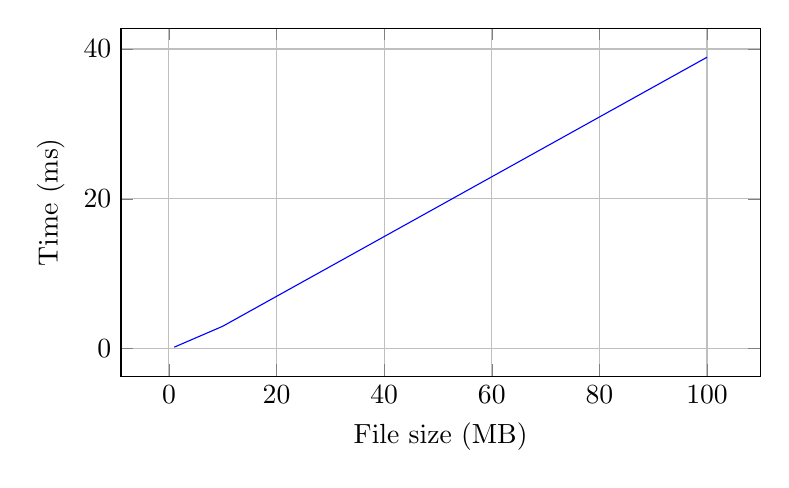
\begin{tikzpicture}
    \begin{axis}[
      xlabel={File size (MB)},
      ylabel={Time (ms)},
      grid=major,
      width=0.8\textwidth,
      height=6cm,
    ]
    \addplot[mark=., blue] coordinates {
      (1, 0.21614)
      (10, 3.002728)
      (100, 38.900041)
    };
    \end{axis}
  \end{tikzpicture}
  \caption[]{Time required to create the challenge response for PoR on the Keeper side, without reading the file from disk.}
  \label{fig:por-keeper}
\end{figure}

\subsection{Attacks on the reputation system}

One of the questions we want to answer in this thesis is if a reputation system based on a ledger store is secure.
In other words, can we use the ledger to store the reputation of the peers in the network and be sure that
the reputation is not tampered with, and
does introducing a reputation system based on a ledger store perhaps introduce new vulnerabilities to the system?
To answer this question we need to talk about possible attacks on the reputation system.

Ranking peers in the network based on their reputation means that 
having higher reputation gives merits to a peer.
Therefore, peers might try to cheat the system in order to increase their reputation.

We will discuss the following attacks:
\begin{enumerate}
    \item \textbf{Increasing reputation attack} --- a peer tries to increase its reputation.
    \item \textbf{Decreasing reputation attack} --- a peer tries to decrease another peer's reputation.
\end{enumerate}

\textbf{Increasing reputation attack} is when a peer tries to increase its reputation by
cheating the system.
The reputation is stored in a ledger, which means that any changes to the data are recorded.
If a peer tries to increase its reputation, the other peers in the network can detect this by
checking the ledger's history.
This leaves the attacker one option - award itself reputation, i.e., a Sybil attack.
Since reputation is only awarded for storing data and performing audits, the attacker could join the network
with multiple identities and perform audits on itself.
This wouldn't work, because audits are performed on a rotating basis, i.e., each cycle a peer audits only a 
certain subset of the network.
If an attacker tries to audit itself not following the cycle, the other peers in the network can detect this,
because the audits are stored in the ledger as well and can be checked by other peers in the network.
This leads us to the situation where if a peer tries to perform a Sybil attack and cheats, it will be detected by
the network.
If the peer tries to perform a Sybil attack and doesn't cheat,
it will simply contribute to the network as any other peer.

\textbf{Decreasing reputation attack} is when a peer tries to decrease another peer's reputation.
We can apply the same reasoning as for the increasing reputation attack.
Directly increasing another peer's reputation is not possible, because the ledger is immutable and keeps track of
all the changes.
The second way to decrease reputation is to perform audits on the peer and fail them.
Since the audits' results are stored in the ledger, the other peers in the network can check the results,
and see if the peer is being honest.

As a conclusion - while attacks are possible, they are easily detected by the network
and do not pose a threat to the system as a whole.

\section{Audits}

Audits are a key part of the reputation system.
They check if the peers are storing the data they claim to store.
The audits are performed by the Verifier against the Keepers and the results are stored in the ledger.
The audit process follows the PoR protocol, where the Verifier sends a challenge to the Keeper,
and the Keeper responds with the proof, which the Verifier checks.

Verifiers perform audits on a rotating basis, i.e., each cycle a Verifier is responsible for auditing
a subset of the files in the network.
e.g., If we have two Verifiers, in cycle one Verifier A audits the first half of the key space,
and Verifier B audits the second half.
In cycle two, they switch --- Verifier A audits the second half and Verifier B audits the first half.
The length of the cycle depends on how much data is in the system --- this will determine
how much time it takes to audit all the files in the network.

Upon completing the audit of all the files, the Verifier stores the results in the ledger.
The results could look something like this:
\begin{verbatim}
  {
      "keeper": "A",
      "file": "1.txt",
      "result": "success",
      "cycle": 1,
  }
\end{verbatim}

Upon a successful audit the Keeper gains reputation points.
Upon a failed audit the Keeper loses reputation points.
The Verifier also gains reputation points for performing the audit.

These 3 changes in reputation are stored in the ledger and can be checked by other peers in the network.
We discussed attacks where the Keeper aims to adjust its reputation in the previous section.
We will now look into how we can stop the Verifier from misbehaving.

The Verifier can misbehave in the following ways:
\begin{enumerate}
    \item \textbf{Not performing audits} --- the Verifier claims to perform audits, but does not.
    \item \textbf{Performing audits incorrectly} --- the Verifier performs audits, but does not check the results correctly.
    \item \textbf{Accusing the Keeper of not storing the data} --- the Verifier accuses the Keeper of not storing the data, but the Keeper is storing the data.
\end{enumerate}

\textbf{Not performing audits} can be caught by inspecting the result of the audits,
which is stored in the ledger.
In other words, in a given cycle, when a Verifier is auditing a set of Keepers,
it will also audit the Verifiers that were previously responsible for auditing the Keepers.
These audits will be to compare the results of the current Verifier with the results of the previous Verifiers,
which can be found in the ledger.

\textbf{Performing audits incorrectly} can be caught in the same way as not performing audits.

\textbf{Accusing the Keeper of not storing the data} can be caught in the next cycle
when the next Verifier audits the same Keeper.
If the Keeper is storing the data, the audit will pass, and the Verifier that accused the Keeper
will have its reputation reduced.
If the Keeper is not storing the data, the audit will fail, and the Keeper will have its reputation reduced.

In conclusion, if we want to introduce Verifiers and allow each peer in the system to be a Verifier,
we need to ensure that the Verifiers are performing their duties correctly,
similarly to how we ensure that the Keepers are storing the data correctly.
In this case we cannot use PoR, but instead will perform simple audits on the Verifiers,
by comparing the other Verifiers' results with the current Verifier's results.
We are assuming that the current Verifier is one that is honest and is performing the audits correctly.

The downside of this approach is that if there are more than 50\% malicious Verifiers in the network,
they can collude and cheat the system,
so we require the majority of the Verifiers to be honest.

\section{Ledger}

The ledger is used as a catalog for the files stored in the network ---
it stores contracts, which state the key of the file, what peer is storing the file,
and the expiry date of the file.
The ledger also stores the reputation of the peers in the network.

In the previous section we discussed how the ledger is used to store the results of the audits.
These results could be very large, if we have many files in the network.
The most basic way to store the results is to store them as a list of JSON objects:

\begin{verbatim}
  {
      "keeper": "A",
      "file": "1.txt",
      "result": "success",
      "cycle": 1,
  }
\end{verbatim}

To optimize the storage of the results, we can store only the failed audits.
We can also only store the contract ID, which is a reference to the file being stored, and the peer ID
where it is stored.
Finally, we could store the results in the System itself and only store the signed hash of the results in the ledger.
This is particularly useful if we want to use a blockchain as the ledger, because then we want to
store as little data as possible in the blockchain, so it does not grow too large.

Ideally the ledger should be a blockchain as it is a form of distributed ledger,
that all peers in the network can access and check.


% The one exception is storage attacks.
% No decentralized network has a solution for storage attacks.

% \subsection{Storage attacks}
% \label{section:storage-attacks}

% Storage attacks are the main focus of this thesis.
% They are mostly ignored by the literature, because decentralized networks are often designed to
% drop old files based on some criteria, such as popularity or age.
% This is done to save space and to keep the network up to date.
% However, if we want durable storage, we need to address these attacks.

% Storage attacks can be classified into two categories:
% \begin{enumerate}
%     \item \textbf{Data availability attacks} --- an attacker claims to store data, but does not.
%     \item \textbf{Data integrity attacks} --- an attacker claims to store data, but stores different data.
% \end{enumerate}

% Checking if a node stores the data it claims to store can be as simple as asking the node to return the data.
% However, this is a very inefficient and bandwidth-consuming method.
% Ideally, we would like to reduce the amount of traffic between nodes and still be able to check
% if the data is stored correctly.

\wtf{TODO: format this explanation at the beginning of the chapter - explaining how the reputation system works}

Filecoin uses the coin as payments, we want to use the coin as a stake.
The coin indicates reputation, not wealth.
We want to trade storage for storage, not storage for money.
i.e., using coins to trade trust/credibility, not work done.
Filecoin makes the assumption that PoR protocols do not check the whole file,
which is not true in the protocols we are looking at.
Filecoin also mentions two types of new attacks:
Sybil attack, where the malicious peers create multiple identities but store the same data in 1 place.
And Outsourcing attacks --- malicious peers claim to be able to store more data than they actually can,
by storing the data elsewhere (e.g., in the network) and rely on quickly fetching it when requested.
Maybe we can use timeouts for the audits to prevent this --- because PoR should be very fast (no network delay).
Proof of Spacetime can be used as well --- require the server to run PoR every X time and then use some form Of
chained hashes or signatures to collect all the proofs and verify them in a single audit (not sure If
this works with the current PoR protocols, but it's an idea).
